El diseño de este proyecto surge de un proceso iterativo en el que se han ido descubriendo los requerimientos poco a poco y trabajando para satisfacerlos de la forma más efectiva posible. Esto se ha traducido en un diseño simple, que no intenta solucionar problemas teóricos que nunca se darán en la práctica, a la vez que ofrece una base extensible capaz de adaptarse a cualquier nuevo requerimiento que pudiera surgir para quien desee extender su funcionalidad. De esta manera, hemos logrado crear una aplicación sencilla de operar para los usuarios y fácil de gestionar para sus administradores.

En este capítulo nos adentraremos en el diseño de GH2GR, comenzando con una visión general de todo el sistema, para luego analizar sus componentes en detalle.
\section{Traducción entre GoRace y Github Classroom} \label{title:mapping-gorace-gh}
GH2GR es una aplicación que se encarga de trasladar los eventos ocurridos en una plataforma a otra. Así pues, lo primero que debemos discutir sobre su diseño es cómo traduce e interpreta los recursos y eventos de las plataformas con las que interactúa y cómo realiza la traducción de una a la otra. Para esto, necesitamos entender los términos que utiliza cada plataforma.

En GoRace, cada experiencia didáctica, ya sea una asignatura, un curso, un torneo, etc., se empaqueta en lo que ellos denominan una carrera. Las carreras son contenedores de nivel superior y están completamente aisladas entre sí. Dentro de las carreras, los participantes pueden completar actividades para avanzar. GoRace evalúa el desempeño de cada participante en una actividad mediante los valores obtenidos en las variables de dicha actividad. GoRace descompone cada actividad en variables, que son básicamente contenedores de puntuaciones con un rango posible de valores. Por ejemplo, podríamos tener una variable que admite valores del 0 al 10 y otra del 0 al 100. Gracias a estos rangos, es posible determinar cuán satisfactorio es el valor almacenado en la variable, pues no representa lo mismo un 10 en la primera variable, que indicaría un éxito absoluto, que en la segunda variable, donde sería un resultado paupérrimo.

Por otro lado, GitHub Classroom encapsula cada experiencia en lo que llama \textit{classrooms} o clases. A su vez, estas clases contienen \textit{assignments} o tareas que, como su nombre indica, son las distintas tareas que el docente asigna a los alumnos. Dentro de cada tarea, el docente puede definir cuantas pruebas automatizadas de evaluación considere necesarias, asignando una puntuación a cada una de ellas. Posteriormente, cuando los alumnos hagan sus entregas, GitHub Classroom sumará las puntuaciones de cada prueba superada por el alumno y le presentará el total junto al máximo posible si hubiera superado todas las pruebas.

Ahora, al trasladar el avance de los alumnos desde GitHub Classroom hasta GoRace, encontramos natural traducir las \textit{classrooms} en carreras y los \textit{assignments} en actividades. Efectivamente, esta fue la decisión tomada, ya que consideramos que de esta forma resultaría más intuitivo para los usuarios. No obstante, aunque podría parecer tentador relacionar las pruebas automatizadas de evaluación con las variables de GoRace, decidimos optar en contra. Proceder de esa manera resultaría en una pérdida de expresividad, ya que las variables de GoRace admiten un rango de valores, mientras que las pruebas automatizadas son binarias; estas pruebas solo pueden ser superadas o no serlo, y proporcionarán su puntuación únicamente si son superadas.

Para resolver este dilema, GH2GR define un método que permite crear múltiples agrupaciones de pruebas automatizadas de evaluación dentro de una misma actividad a través de un prefijo en el nombre de la prueba con el formato de \textit{[Nombre Variable]}. Son estos grupos entonces los que se asignan a las variables de GoRace. Cada grupo tiene un rango definido de \([0,N]\), siendo \(N\) la suma de las puntuaciones de cada una de las pruebas del grupo. El valor que cada alumno obtendrá en cada grupo será la suma de las puntuaciones de todas las pruebas que haya superado.

\begin{figure}
    \centering
    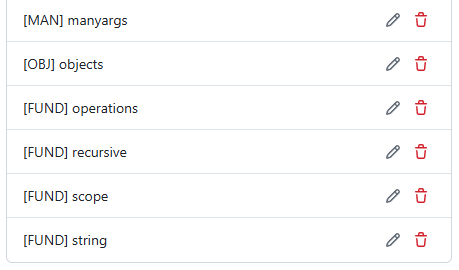
\includegraphics[width=0.5\linewidth]{images/variable-groups-autograding-tests.png}
    \caption{Ejemplo de pruebas automatizadas de evaluación agrupadas en Github Classroom. En la imagen se muestran tres grupos: FUND, OBJ y MAN.}
    \label{fig:variable-groups-autograding-tests}
\end{figure}

Ahora que hemos expresado los grupos en los mismos términos que las variables de GoRace, es sencillo ver cómo es posible una traducción sin pérdida de expresividad. Pues tan solo requerimos hacer una regla de tres para transformar el valor del rango del grupo de pruebas al de la variable de GoRace. El único problema de este acercamiento es que, a la fecha de la escritura de este documento, no es posible extraer de GoRace cuál es el rango de la variable. Para bordear este problema, GH2GR asume que las variables de GoRace tienen un rango de cero a cien \([0,100]\). Si bien con este compromiso se pierde un poco de flexibilidad, consideramos que ofrece expresividad suficiente para cualquier aplicación.


\section{Diseño a alto nivel del sistema}
\begin{figure}
    \centering
    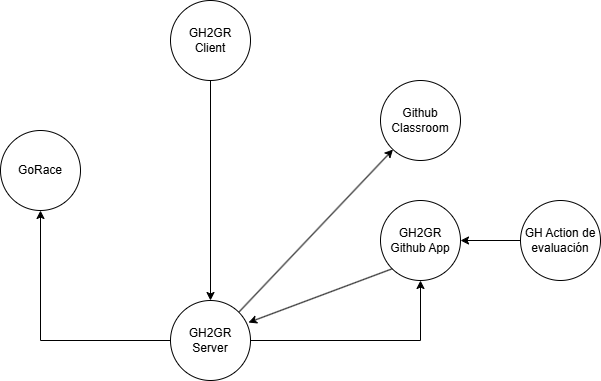
\includegraphics[width=0.75\linewidth]{images/comunicacion-componentes.png}
    \caption{Diagrama que muestra los componentes a alto nivel que interactúan en el funcionamiento de GH2GR. Los círculos representan componentes, mientras que las flechas indican que un componente (el que origina la flecha) puede iniciar comunicación con otro (al que apunta la flecha).}
\end{figure}
En una experiencia que utiliza GH2GR podemos encontrar los siguientes componentes base:
\begin{itemize}
    \item \textbf{GH2GR Server}: Es el componente principal de GH2GR. Este componente se encarga de extraer los resultados desde GitHub y brindarlos a GoRace. Adicionalmente, ofrece una \acrshort{API} para su gestión.
    \item \textbf{GitHub App}: Este constructo nos proporciona las credenciales para interactuar con la \acrshort{API} de Github y así poder acceder a los recursos que se esconden detras de esta.
    \item \textbf{GitHub Classroom}: Alberga toda la información relativa a las tareas, agrupaciones de alumnos, etc. Desde aquí el profesorado crea las distintas tareas y define las pruebas automatizadas de evaluación.
    \item \textbf{GitHub Action de evaluación}: Esta \textit{Action} se ejecuta automáticamente cuando un alumno publica algún cambio en su repositorio, ejecutando las pruebas de automatizadas de evaluación definidas por el profesor y ofreciendo los resultados en un formato de fácil lectura para GH2GR Server.
    \item \textbf{GH2GR Client}: Utilidad de línea de comandos que permite al profesor gestionar la integración por medio de la \acrshort{API} de GH2GR Server y generar el \textit{workflow}\cite{githubUnderstandingActions} para la Github Action de evaluación.
    \item \textbf{GoRace}: Es la plataforma de ludificación. Recibe las actualizaciones de GH2GR Server y las utiliza para avanzar la experiencia lúdica según los designios del profesorado.
\end{itemize}
Para entender mejor cual el rol de cada una de las partes, es conveniente explicar que ocurre desde que un alumno realiza un cambio a su repositorio hasta que el resultado de este se ve reflejado en GoRace:

\begin{figure}
    \centering
    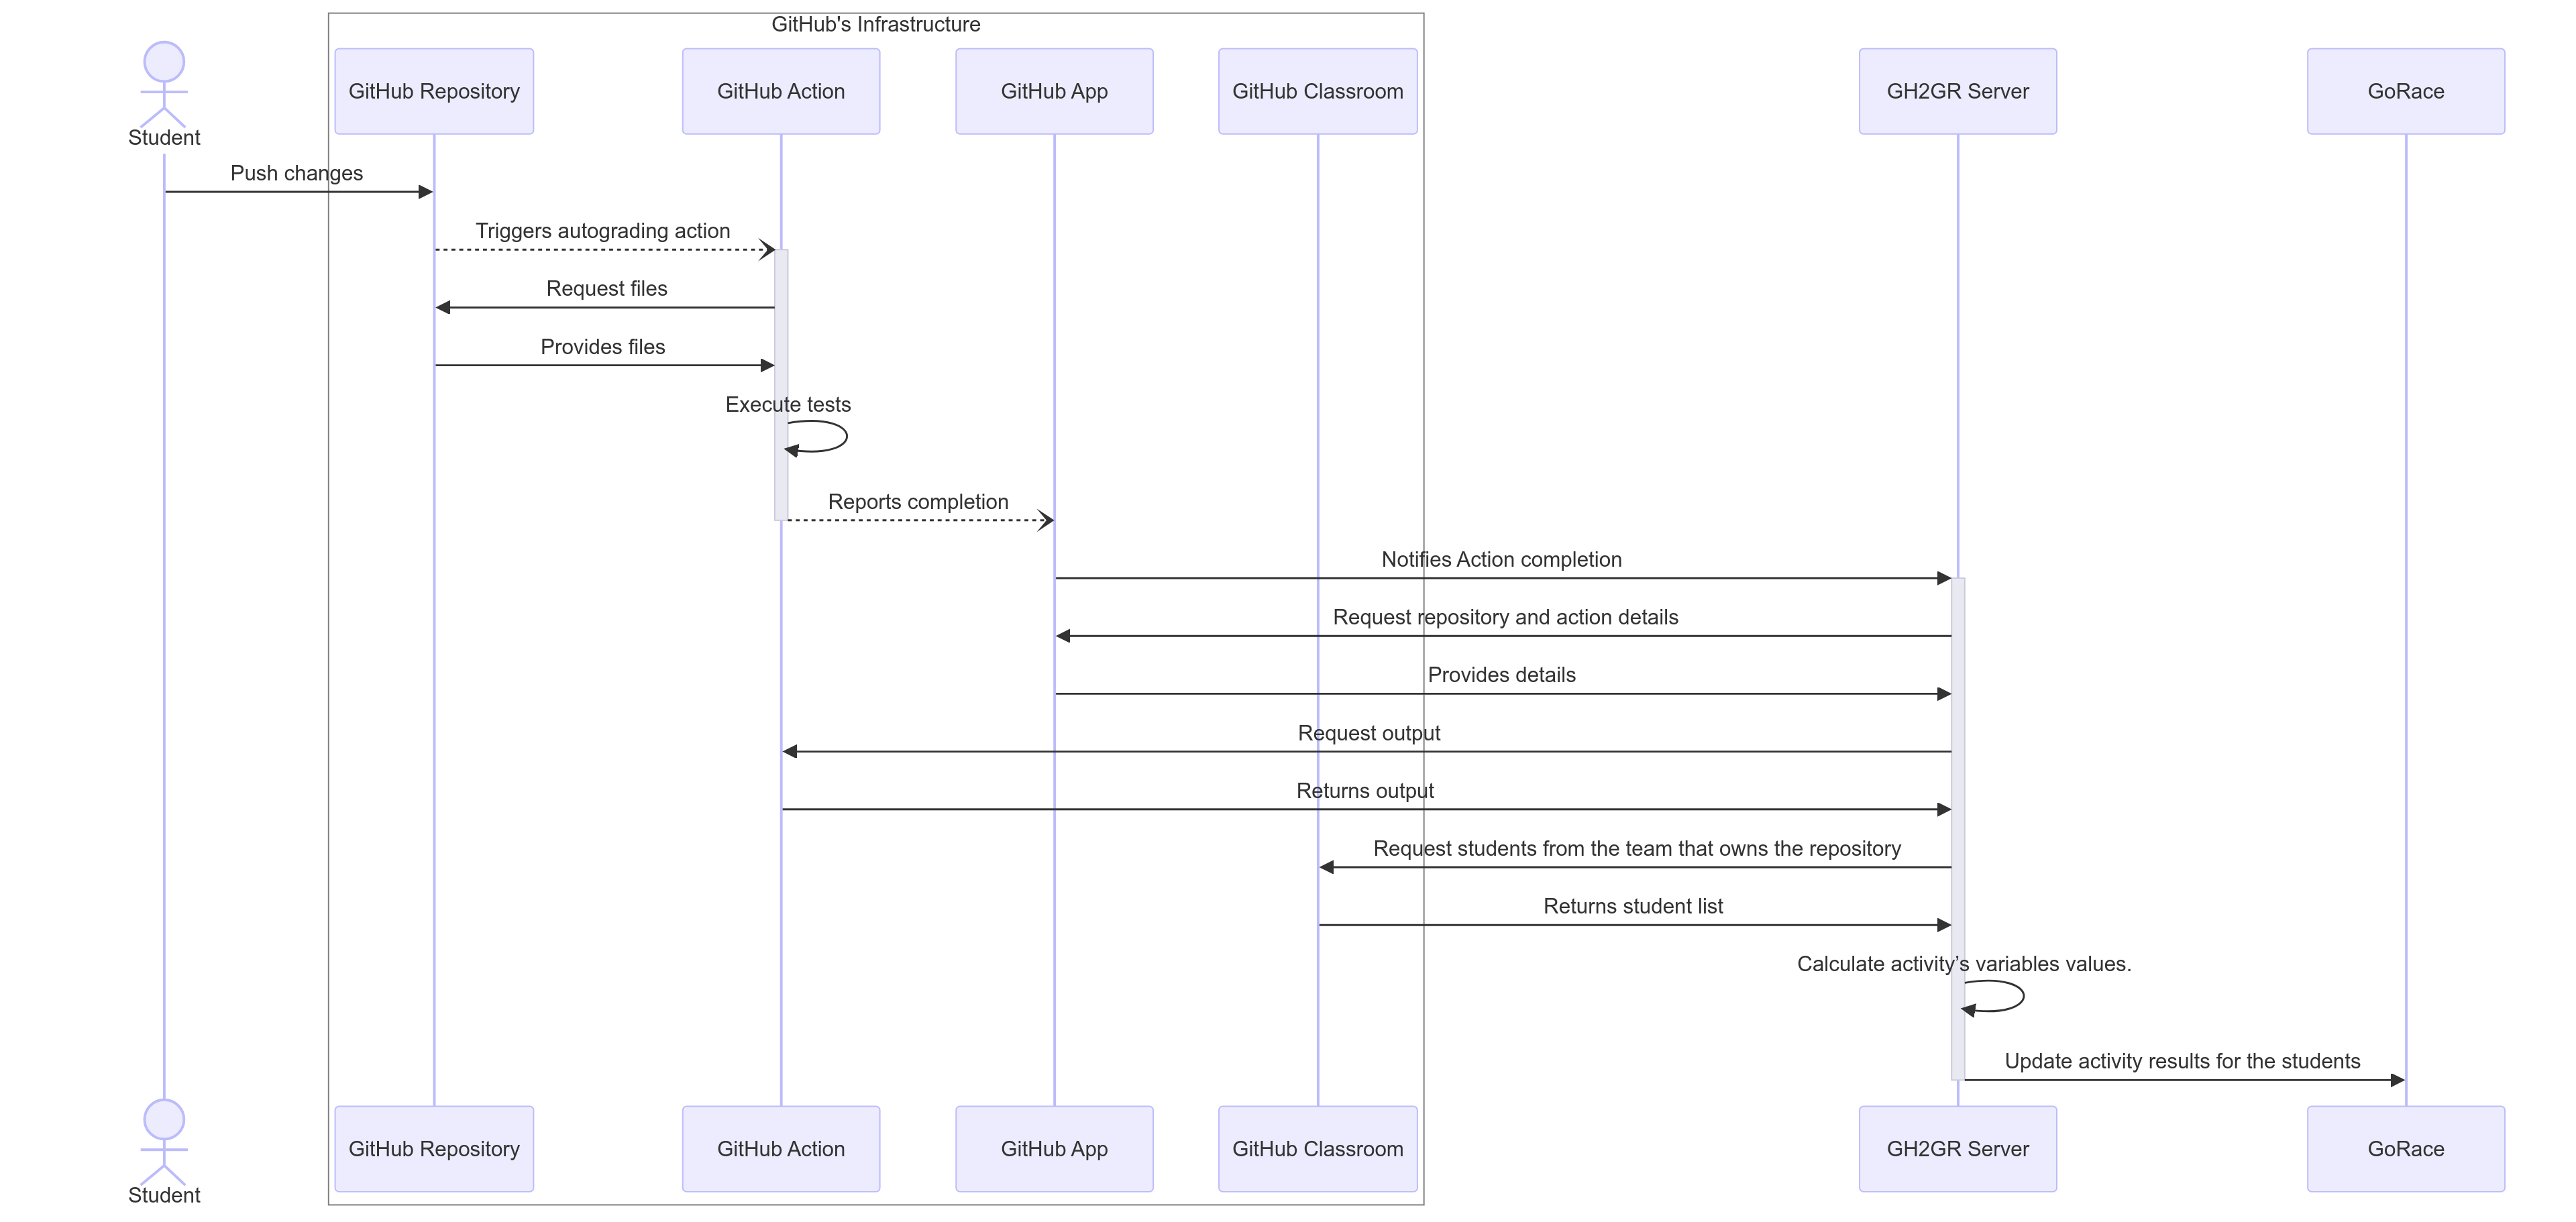
\includegraphics[width=\linewidth]{images/flow-after-push.png}
    \caption{Diagrama de flujo de los eventos que ocurren tras la realización un \textit{push}. TODO: LEYENDA DE FLECHAS}
    \label{fig:enter-label}
\end{figure}

Lo primero que ocurre cuando un alumno sube sus cambios a su repositorio en GitHub es que la plataforma ejecuta la Github Action de evaluación. Esta, a su vez, lee el fichero de configuración que creó GitHub Classroom cuando el profesor definió las pruebas automáticas de evaluación. Tras consultar el fichero, la Action ejecuta las pruebas una por una y produce como salida un \acrshort{JSON} detallando cada prueba ejecutada, su puntuación de ser superada y si la prueba en cuestión fue superada o no. Además, esta salida añade algunos detalles como la carrera a la que pertenece, la actividad y el identificador del \textit{assignment} de GitHub Classroom al que pertenece.

La GitHub App está configurada de tal forma que monitorea la ejecución de las Github Actions. Así, a través de un \textit{webhook}, es decir, una llamada \acrshort{HTTP}, es capaz de avisar a GH2GR Server de este evento, otorgándole, además, contexto como el identificador de la ejecución y el repositorio donde ocurrió. Con esa información, el servidor utiliza sus credenciales de la App de GitHub para acceder a la salida de la Github Action. Una vez ha leído el \acrshort{JSON}, accede a la \acrshort{API} de GitHub Classroom y busca a todos los alumnos relacionados con el repositorio, ya que GitHub Classroom permite que las actividades se realicen en equipo y, en tal caso, asigna un solo repositorio a todos los miembros. Luego, agrupa las pruebas en las distintas variables a partir del texto entre corchetes que se usa como prefijo en cada prueba. Una vez agrupadas, se calcula la puntuación máxima de cada grupo sumando todos los puntos que pueden dar las pruebas que los componen y cuántos se han obtenido por pruebas superadas. Es ahora cuando el servidor aplica una regla de tres para ajustar el resultado al rango de las variables en GoRace, que, como se comentó antes, se espera que sea de cero a cien. Finalmente, el GH2GR Server actualiza el resultado de la actividad con los valores de las variables obtenidos para todos los alumnos partícipes del repositorio.

\section{Sobre la GitHub App}
Como ya se comentó con anterioridad, la GitHub App no es una aplicación per se, pues no es algo que podemos programar. En su lugar, es un constructo que ha creado GitHub para agrupar y dar nombre a los permisos y credenciales que necesita una aplicación para interactuar con la API de GitHub y para escuchar los eventos que puedan surgir en la plataforma.

A fin de que la aplicación esté autorizada para acceder a los recursos (ej. Repositorios, ejecuciones de GitHub Actions, etc.) necesarios para su correcto funcionamiento, la GitHub App debe ser "instalada", utilizando la terminología de la propia GitHub, en la organización en GitHub utilizada para crear el \textit{classroom}. En términos más comunes, la GitHub App tiene que ser autorizada para acceder a los recursos que se esconden bajo el manto de la organización.

\begin{figure}
    \centering
    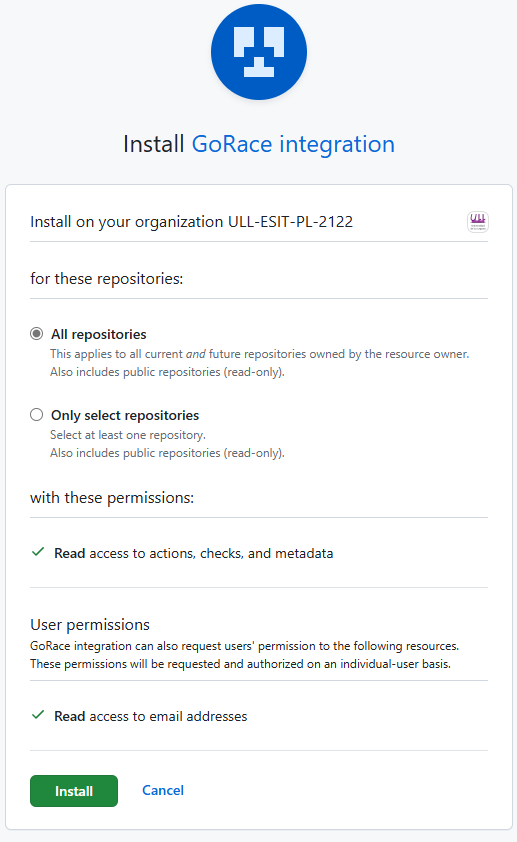
\includegraphics[width=0.4\linewidth]{images/install-screen.png}
    \caption{Pantalla de instalación de la GitHub App en una organizaicón.}
\end{figure}

Como buena práctica de seguridad, se ha tratado de reducir los permisos que solicita la GitHub App asociada a GH2GR al mínimo imprescindible. Es por esto que nuestra GitHub App no requiere de ningún permiso de escritura y solo requiere acceso de lectura de los siguientes permisos:
\begin{itemize}
    \item \textbf{Metadata}: Permite listar los repositorios, colaboradores y otros datos superficiales. Es un permiso básico que GitHub obliga a todas las \textit{apps} a solicitar.
    \item \textbf{Actions}: Permite acceder a información de las GitHub Actions: cuáles hay en un repositorio, cuándo se lanzan, cuándo terminan, etc. No permite acceder a la salida de una ejecución de una GitHub Action en particular.
    \item \textbf{Checks}: Permite acceder a la salida de las GitHub Actions.
\end{itemize}

Además de permitir acceder a la API de GitHub, la GitHub App nos permite ser avisados de eventos, como, por ejemplo, cuando se completa la ejecución de una GitHub Action, a través de un mecanismo de \textit{webhook}. Un webhook es un mecanismo de mensajería en tiempo real empleado para automatizar la comunicación entre aplicaciones. Cuando se produce un evento predefinido en un sistema de origen (por ejemplo, una nueva entrada de datos o la finalización de una tarea), se activa una solicitud \acrshort{HTTP} que envía los datos relevantes (\textit{payload}) a una \acrshort{URL} designada en un sistema receptor. Esto permite que las aplicaciones reaccionen rápidamente a los eventos sin necesidad de un sondeo constante, lo que fomenta un flujo de trabajo más eficiente.\cite{redhatWhatWebhook}

\section{Sobre la GitHub Action}
La GitHub Action es un programa autocontenido que se ejecuta en la infraestructura de GitHub cuando un alumno sube un cambio al repositorio. Este programa, de hecho, es un \textit{fork} del que utilizaba la propia GitHub \cite{githubGitHubEducationautograding}.

La Action está escrita en TypeScript \cite{typescript} y está diseñada para ejecutarse sobre NodeJS \cite{nodejs}. Tras leer el fichero \textit{autograding.json}, la Action ejecuta las pruebas de forma secuencial, ejecutando el comando que se especifica en cada una y comparando la salida obtenida con la esperada para superar la prueba. Las comprobaciones que se pueden hacer son variadas, pues se puede observar el código de salida \cite{exitcode} o se puede comparar la salida estándar esperando una salida en concreto, que la salida contenga un fragmento de texto concreto o que la salida satisfaga una expresión regular.

Tras ejecutar las pruebas y determinar su resultado, la GitHub Action produce como salida un documento \acrshort{JSON} con la siguiente estructura:
\begin{itemize}
    \item \textbf{\textit{activity}}: Nombre de la actividad en GoRace a la que alude el repositorio.
    \item \textbf{\textit{assignmentId}}: El identificador del \textit{assignment} en GitHub Classroom. Es un valor numérico entero.
    \item \textbf{\textit{race}}: El nombre de la carrera en GoRace.
    \item \textbf{\textit{results}}: Vector conteniendo los resultados de cada una de las pruebas.
    \begin{itemize}
        \item \textbf{\textit{name}}: El nombre de la prueba automatizada de evaluación.
        \item \textbf{\textit{failed}}: Si la prueba se ha pasado con éxito o no. Valor booleano, verdadero si la prueba ha fallado o falso si se ha superado con éxito.
        \item \textbf{\textit{points}}: Cuántos puntos vale la prueba automatizada de evaluación. Valor numérico entero.
    \end{itemize}
\end{itemize}

Se ha escogido utilizar \acrshort{JSON} porque es un formato de datos ligero y de texto plano, lo que facilita su lectura y escritura tanto para humanos como para máquinas. Su estructura, basada en pares clave-valor y vectores, es intuitiva y directa, lo que simplifica la serialización y deserialización. Estas características han posibilitado que \acrshort{JSON} se transforme en un lenguaje omnipresente que cuenta con utilidades para ser procesado en casi cualquier lenguaje de programación \cite{jsonJSON}. Estos puntos hacen que \acrshort{JSON} sea un lenguaje ideal para la tarea que tenemos entre manos, pues nos permite fácilmente revisar la salida del programa para detectar cualquier posible fallo a simple vista y no nos limita en las tecnologías que podemos usar en el resto del sistema. Además, el soporte para \acrshort{JSON} se encuentra integrado de forma nativa en NodeJS \cite{ecma262}.

\section{GH2GR Server en detalle}
El componente de servidor de GH2GR es el corazón de la aplicación y donde se concentra la mayor parte del trabajo. Es responsable de hacer la transformación real de la información obtenida de GitHub y traducirla para que GoRace la pueda entender.

A este componente lo denominamos servidor porque su función principal es servir como un servidor \acrshort{HTTP} que recibe los eventos del \textit{webhook} de la GitHub App y presenta una \acrshort{API} de gestión.

El \textit{webhook} está diseñado para seguir la especificación de GitHub. Es decir, se trata de un \textit{endpoint}, es decir, una \acrshort{URL}, que recibe peticiones \acrshort{HTTP} de tipo POST con la información del evento en el cuerpo de la petición codificada en formato \acrshort{JSON}. Adicionalmente, el servidor espera que en la petición \acrshort{HTTP} se encuentre la cabecera ''X-Hub-Signature-256''. Esta cabecera debe contener una firma \acrshort{HMAC}\cite{rfc2104} utilizando el hash SHA-256\cite{Dang2015} del contenido del cuerpo de la petición firmado con un secreto establecido en la configuración de GitHub y proporcionado a GH2GR Server a la hora de su arranque. Si el servidor no es capaz de verificar la validez de la firma de la petición, la petición al completo será descartada y el servidor retornará una respuesta inmediata con el código \acrshort{HTTP} 400 \textit{Bad Request}, indicando que la petición es inválida y el servidor se niega a procesarla \cite{rfc7231}. Esto se hace para evitar que un atacante que haya descubierto la \acrshort{URL} del \textit{endpoint} sea capaz de engañar al sistema enviando eventos falsos.

Lo anterior resume el diseño del \textit{webhook}, pero se puede encontrar más información sobre la información que recibe el \textit{webhook} en la documentación de GitHub del evento de \textit{workflow\_run} \cite{githubWebhookEvents} y sobre la validación en la sección de la documentación dedicada a la validación del \textit{webhook} \cite{githubValidatingWebhook}.

En cuanto a la \acrshort{API} de gestión, hablaremos de ella más en detalle en el apartado \ref{api-gesion}.
\subsection{Estructura del código}

GH2GR Server está escrito en el lenguaje de programación Go\cite{goProgrammingLanguage}. Esto afecta profundamente a cómo está estructurado, pues la estructura del proyecto está en parte moldeada por las funcionalidades, limitaciones y el paradigma del lenguaje, así como por lo que le resulta idiomático.

Go, también conocido como Golang, es un lenguaje de programación compilado de tipado estático diseñado por Google. Notable por su simplicidad y eficiencia, Go proporciona un potente modelo de concurrencia a través de \textit{goroutines} y canales, lo que permite el desarrollo de aplicaciones altamente concurrentes y paralelas\cite{stackoverflowWhatapossGreat}. Además, cuenta con un colector de basura que simplifica la gestión de memoria\cite{golangGuideGarbage}. El lenguaje fue elegido para este proyecto por las siguientes razones (sin orden específico): su simplicidad, la familiaridad del alumno con este, su popularidad en herramientas que interactúan con GitHub, incluyendo la propia GitHub CLI\cite{githubGitHubClicli}, la multitud de librerías disponibles para este fin, y su enfoque en concurrencia que permite desarrollar un servidor eficiente capaz de gestionar múltiples peticiones de forma simultánea de manera sencilla.

Go es un lenguaje ligeramente estricto a la hora de organizar código. En él, múltiples archivos en una misma carpeta conforman un paquete. Dentro de un mismo paquete no existe una barrera que separe el código privado del público, pudiendo cualquier archivo acceder a todas las funciones de cualquier otro. No obstante, cuando hablamos de acceder a lo definido en un paquete externo, Go sí ofrece una separación clara entre lo público, al cual podremos acceder, y lo privado, cuyo acceso nos será prohibido por el compilador. Para acceder a la interfaz pública de otro paquete, tendremos que importarlo, es decir, declarar que queremos hacer uso del mismo, marcándolo como una dependencia. Aquí encontramos una de las peculiaridades del lenguaje, pues el grafo de dependencias de paquetes debe ser acíclico. En otras palabras, un paquete no puede importar ningún paquete que intente importarlo, o que sus dependencias intenten importarlo.

Finalmente, debemos discutir el paradigma de programación del lenguaje, ya que, por supuesto, esto también afecta a cómo estructuramos nuestro código. En este aspecto, es complicado hacer un corte claro y fino del paradigma al que pertenece Go. Go es principalmente un lenguaje imperativo con elementos de orientación a objetos sin llegar a serlo puramente\cite{goFAQOOP}, y también cuenta con ciertos elementos más propios de la programación funcional\cite{goCodewalkFirstClass}.

Ahora que hemos terminado de discutir cómo afecta el lenguaje a la organización del código, podemos pasar a hablar de los principios que han guiado la estructura de este. Dicha estructura está fuertemente inspirada por el modelo \acrshort{MVC}\cite{universitetetiosloTrygveMVC}, contando con un controlador que responde a los eventos externos y un modelo que engloba la lógica de negocio. Además, tiene una influencia de la arquitectura hexagonal\cite{cockburnHexagonalArchitecture}, ya que se han diseñado capas que aíslan a la lógica de negocio y evitan que dependa de recursos externos, aprovechando al máximo el Principio de Inversión de la Dependencia\cite{Martin2002-yw}.

El paquete principal de GH2GR es el paquete \textit{models}. Este paquete contiene los tipos abstractos de datos que se utilizan para contener la información en toda la aplicación, el código que se encarga de validar sus valores y las operaciones sobre estos datos que no requieren de ningún recurso externo.

A continuación, nos encontramos con el paquete \textit{services}. Este paquete alberga las operaciones o procesos que debe realizar la aplicación. Por ejemplo, si decimos que GH2GR permite actualizar la información que tiene el servidor sobre una carrera, en este paquete nos encontraremos una función que encapsula esta funcionalidad. Esta función se encargará de revisar que la carrera en cuestión existe, que el docente que está intentando hacer la modificación es dueño de la carrera y de asegurarse de que la modificación es válida. No obstante, este paquete también se puede ver como una extensión de \textit{models} pues contiene solo lógica de negocio. Tampoco se le permite a este paquete tener dependencias externas más allá de \textit{models}, por lo que se vale de interfaces definidas por sí mismo o por \textit{models} para interactuar con recursos externos. El motivo de que este sea un paquete separado de \textit{models} es tan sencillo como el deseo de evitar que \textit{models} acabe albergando demasiado código. Esta es una ocurrencia tan habitual que a esta pequeña variación de \acrshort{MVC} se le ha apodado como \acrshort{MVCS}\cite{mvcs}.

El siguiente gran paquete del que tenemos que hablar es el paquete \textit{controllers}. Podemos ver este paquete como una capa de traducción entre nuestra \acrshort{API} \acrshort{HTTP} (TODO insertar ref) y las operaciones que tenemos definidas en \textit{services}. Así pues, en este paquete hallaremos todo el código responsable de manejar rutas, verbos y cabeceras \acrshort{HTTP}, así como de la serialización y deserialización de los distintos documentos \acrshort{JSON} que representan la información de nuestros modelos.

Los paquetes que restan son paquetes más utilitarios, con un nombre que identifica el propósito de cada paquete, siguiendo las recomendaciones de estilo de Go\cite{goPackageNames}. Ejemplos de estos son el paquete \textit{database}, que tiene el código que interactúa directamente con la base de datos; el paquete \textit{cli}, que contiene utilidades para construir la interfaz de línea de comandos; el paquete \textit{gorace}, que traduce las partes relevantes de la \acrshort{API} \acrshort{HTTP} de GoRace a una \acrshort{API} Go; el paquete \textit{github}, que cumple una función similar al paquete \textit{gorace}, pero para GitHub y GitHub Classroom, etc.

\subsection{Los tipos abstractos de datos principales}
Ahora examinaremos cuáles son los \acrshort{ADT} principales del programa, que sirven para almacenar y transportar la información más importante entre las distintas capas de la aplicación.

El primero que nos encontramos es el que representa la información que necesitamos saber sobre la carrera en GoRace, adecuadamente llamado \textit{Race}. Este tipo cuenta con los siguientes campos:
\begin{itemize}
    \item \textbf{ID}: Tipo entero. Identificador interno de la carrera.
    \item \textbf{JWT}: Token de acceso para la API de GoRace.
    \item \textbf{Name}: Tipo texto. El nombre de la carrera.
\end{itemize}

El primer campo es un simple identificador numérico, que sirve para distinguir de forma inequívoca una carrera en cuestión del resto. Por su lado, el campo de nombre es un simple apodo para la carrera, pensado para que los usuarios puedan identificar rápidamente la carrera sin tener que lidiar con identificadores numéricos. Por último, el campo de \acrshort{JWT} contiene el token proporcionado por GoRace que autoriza a interactuar con la carrera por medio de su \acrshort{API}.

Luego tenemos el \acrshort{ADT} de \textit{User}, que refleja a un usuario directo de GH2GR-Server, es decir, un docente. Los campos que lo componen son los siguientes:
\begin{itemize}
    \item \textbf{ID}: Tipo entero. Identificador interno para el usuario.
    \item \textbf{Username}: Tipo texto. El nombre del usuario.
    \item \textbf{GithubToken}: El token de GitHub del usuario.
\end{itemize}
El campo de ID cumple el mismo rol que el que ya hemos visto. El \textit{Username} es el nombre de usuario único con el cual se puede identificar al docente. Finalmente, el GithubToken es un token personal de GitHub proporcionado por el docente. Este dato es necesario ya que la \acrshort{API} de GitHub Classroom no puede ser accedida por GitHub Apps propiamente, sino que requiere de un token generado por el usuario para la aplicación\cite{ClassroomAPI}. Así pues, como este dato está asociado estrictamente a un usuario, se almacena con los datos propios de este.

Ahora echemos un vistazo a los \acrshort{ADT} que representan los datos que esperamos obtener de GitHub. Primero, tenemos el tipo GithubInput, que cuenta con los siguientes campos:
\begin{itemize}
    \item \textbf{Activity}: Tipo texto. El nombre de la actividad correspondiente en GoRace.
	\item \textbf{Race}: Tipo texto. El nombre de la carrera correspondiente en GoRace.
	\item \textbf{TestResults}: Tipo vector de ScoreInput. Los distintos resultados de las pruebas de evaluación automatizadas.
	\item \textbf{AssignmentId}: Tipo entero. El identificador de la tarea en GitHub Classroom.
\end{itemize}
Como podemos comprobar, esta es la entrada esperada cuando obtenemos la salida de la GitHub Action. Por tanto, los datos que aquí tenemos son los necesarios para ponernos en contexto de qué tarea estamos puntuando, más los resultados que nos proporcionan los valores para calcular la puntuación. Es propio que ahora revisemos el tipo ScoreInput, que contiene los siguientes campos:
\begin{itemize}
    \item \textbf{Name}: Tipo texto. El nombre de una prueba de evaluación automatizada.
	\item \textbf{Points}: Tipo entero sin signo. La cantidad de puntos que proporciona la prueba.
	\item \textbf{Failed}: Tipo booleano. Representa si la prueba ha sido superada (valor falso) o fallida (valor verdadero).
\end{itemize}

Ahora solo nos resta explorar un pequeño \acrshort{ADT} llamado GithubUserMapping, que viene a solventar el problema de que GitHub principalmente nos habla de los usuarios usando nombres de usuario, mientras que GoRace lo hace hablando de correos electrónicos. Y aunque sería posible preguntar por los correos electrónicos a GitHub, esto representaría la necesidad de que los usuarios autorizaran personalmente a la GitHub App a acceder a este detalle y, aun así, sería problemático, pues una cuenta de GitHub permite tener múltiples correos asociados\cite{githubRESTEmail} y habría que determinar cuál es el adecuado. Para esquivar este problema, este tipo representa una asociación que ha hecho el docente de cada nombre de usuario de GitHub del alumnado con un correo electrónico que se usará en GoRace. Por tanto, este tipo se compone de esos dos campos:

\begin{itemize}
    \item \textbf{Username}: Nombre de usuario en GitHub.
    \item \textbf{Email}: Correo electrónico a usar en GoRace.
\end{itemize}

\subsection{La API de gestión} \label{api-gesion}
La \acrshort{API} de gestión permite a un cliente con las credenciales de un docente añadir carreras bajo su cargo y listar, actualizar y eliminar las carreras que tiene asociadas. Además, le permite crear las traducciones de los nombres de usuario de GitHub de los alumnos a correos electrónicos que usar en GoRace. Por último, también le permite consultar y modificar sus datos de usuario en GH2GR-Server. Notablemente, están exentas de la \acrshort{API} las operaciones de crear o eliminar usuarios docentes, pues esto se considera una operación de administrador y, por tanto, solo se pueden realizar a través de la interfaz de línea de comandos de GH2GR-Server directamente.

La \acrshort{API} tiene un diseño \acrshort{HTTP} \acrshort{REST}-like (similar a \acrshort{REST} sin llegar a serlo). Pues tal como pide \acrshort{REST} \cite{REST}, la \acrshort{API} tiene un diseño cliente/servidor, carece de estado, puede ser \textit{cacheable} y puede ser utilizado de forma transparente a través de distintas capas como cachés, servidores proxy o balanceadores de carga. El factor que hace que la \acrshort{API} sea \acrshort{REST}-like y no completamente \acrshort{REST} se encuentra en el uso de la denominada "interfaz uniforme". Si bien la \acrshort{API} cumple con ella en la mayor parte de su extensión, estando orientada a recursos identificados por \acrshort{URI}, utilizando adecuadamente los verbos \acrshort{HTTP} y expresando los errores de forma semántica utilizando los mecanismos de \acrshort{HTTP}, existen unas pocas operaciones que se presentan en un estilo más propio del \acrshort{RPC}, pues hacía más claro su uso. Además, esta funcionalidad ni siquiera se publicita mediante hipermedia, pues se decidió en contra de usar esta para mantener una \acrshort{API} sencilla.

Aunque se haya optado por no hacer una \acrshort{API} completamente \acrshort{REST}, sí que se han hecho esfuerzos para que la \acrshort{API} sea legible tanto por humanos como por máquinas. A fe de esto, todos los recursos se han modelado utilizando JSON-Schema \cite{jsonschemaJSONSchema}. Además, todos los errores son representados con el código de estado \acrshort{HTTP} más adecuado según la RFC 9110 \cite{rfc9110}, acompañado de un cuerpo que detalla el problema en formato de \textit{problem details}, que ofrecen una forma estándar de especificar de forma inequívoca un problema y ofrecer toda la información sobre este que se considere relevante en un formato legible por personas y consumible por máquinas \cite{rfc9457}. Como culmen de este esfuerzo, se ha documentado la totalidad de la \acrshort{API} en el formato OpenAPI 3.1, un formato que permite tanto a humanos como a ordenadores descubrir y comprender las capacidades de un servicio sin necesidad de acceder al código fuente, documentación adicional o inspección del tráfico de red. Cuando se define correctamente a través de OpenAPI, un consumidor puede entender e interactuar con el servicio remoto con una cantidad mínima de lógica de implementación, de forma similar a lo que las descripciones de interfaces han hecho por la programación de bajo nivel \cite{openapisOpenAPISpecification}. En otras palabras, la \acrshort{API} está documentada en un formato que permite la generación automática tanto de páginas de documentación para el consumo humano, como de \acrshort{SDK} para interactuar con ella directamente desde el código de cualquier aplicación cliente. Esta especificación en formato OpenAPI se encuentra en el anexo \ref{openapi-schema} de este documento.

Dado que ya se encuentra anexa a este documento una documentación completa de la \acrshort{API}, no se explorará más sobre ella en este apartado. Aunque sí se mencionará que su diseño fue altamente influido por \acrshort{ADT}, descrito en el apartado anterior, que sirvió como la base para los recursos sobre los que se modela la \acrshort{API}.
\subsection{La base de datos}
Como ya se comentó anteriormente, en el diseño de GH2GR-Server, la base de datos no es un componente irreemplazable y, de hecho, puede ser sustituida por cualquier otro mecanismo con una cantidad moderada y bien acotada de trabajo. No obstante, es cierto que el rol que cumple es crucial: almacenar de forma permanente los datos y permitir recuperarlos de forma eficiente. Para este trabajo, GH2GR-Server solo se ha dotado de la capacidad de usar un sistema gestor de bases de datos.

El sistema gestor de bases de datos que utiliza la aplicación es SQLite en su versión 3. El motivo de esta elección es que, al ser un \acrshort{DBMS} que está integrado en el propio binario de la aplicación y se ejecuta en el mismo proceso que esta, solo necesita como añadido un lugar donde guardar un fichero \cite{sqliteAboutSQLite}. Esto la convierte en la candidata ideal para mantener la línea de diseño orientada a la simplicidad a la hora de administrar y poner en funcionamiento GH2GR-Server. Además de esta ya deseable característica, SQLite nos ofrece un buen rendimiento y transacciones \acrshort{ACID} sobre una interfaz \acrshort{SQL} \cite{sqliteAboutSQLite}, que nos permite modelar cómodamente las relaciones en los datos que almacenamos \cite{Beaulieu2009-jq}.

\subsection{El método de construcción y despliegue} \label{title:gh2gr-server-build-and-deploy}
Como ya se comentó anteriormente, GH2GR-Server está escrito en Go, un lenguaje de programación famoso por su sencilla compilación y por su habilidad de producir un binario sin dependencias externas, facilitando la distribución \cite{goDevelopmentCLI}. No obstante, GH2GR-Server utiliza las funcionalidades de CGo, una utilidad que permite llamar a los compiladores de C para utilizar código programado en este lenguaje \cite{goCGo}. Dado que utilizamos estos compiladores, necesitamos que estén presentes a la hora de construir nuestro programa y, si deseamos compilar para otra plataforma, también necesitaremos tener las capacidades para compilar este lenguaje para la máquina objetivo.

Para reducir la cantidad de software que es necesario para construir el programa y además contar con un método de despliegue estándar, se ha decidido utilizar contenedores OCI, también conocidos por muchos como contenedores Docker \cite{ociFAQ}. Estos permiten definir un entorno replicable, con todas las dependencias, que posibilita la construcción con un solo comando, produciendo no solo el binario, sino que también lo acompaña con todo el entorno que necesita para ser ejecutado correctamente dentro de un \textit{runtime} de contenedores Linux OCI. Esto significa que puede ejecutarse no solo en casi cualquier máquina Linux \cite{mobyReadme, podmanWhatPodman}, sino también en máquinas Windows y Mac OS \cite{dockerDockerDesktop, rancherdesktopIntroductionRancher, podmandesktopIntroductionPodman}.

Las ventajas que nos traen los contenedores no solo se limitan a lo anterior, y es que, usando las palabras del \textit{Docker Captain} Adrian Mouat \cite{dockerAdrianMouat}:


``

Los desarrolladores pueden crear software localmente, sabiendo que se ejecutará de forma idéntica independientemente del entorno del host, ya sea un rack en el departamento de TI, el portátil de un usuario o un clúster en la nube. Los ingenieros de operaciones pueden concentrarse en las redes, los recursos y el tiempo de actividad, y pasar menos tiempo configurando entornos y luchando contra las dependencias del sistema. 
(...)
Los contenedores son una encapsulación de una aplicación con sus dependencias. A primera vista, parecen simplemente una forma ligera de máquinas virtuales (VM): al igual que una VM, un contenedor contiene una instancia aislada de un sistema operativo (SO), que podemos utilizar para ejecutar aplicaciones.

Sin embargo, los contenedores tienen varias ventajas que permiten casos de uso que son difíciles o imposibles con las máquinas virtuales tradicionales:
\begin{itemize}
    \item Los contenedores comparten recursos con el sistema operativo anfitrión, lo que los hace un orden de magnitud más eficientes. Los contenedores pueden iniciarse y detenerse en una fracción de segundo. Las aplicaciones que se ejecutan en contenedores incurren en una sobrecarga mínima o nula en comparación con las aplicaciones que se ejecutan de forma nativa en el SO anfitrión.
    \item La portabilidad de los contenedores tiene el potencial de eliminar toda una clase de errores causados por cambios sutiles en el entorno de ejecución; incluso podría poner fin al viejo refrán de los desarrolladores de "¡pero si funciona en mi máquina!".
    \item La naturaleza ligera de los contenedores permite a los desarrolladores ejecutar docenas de contenedores al mismo tiempo, lo que hace posible emular un sistema distribuido listo para la producción. Los ingenieros de operaciones pueden ejecutar muchos más contenedores en una sola máquina host que utilizando solo máquinas virtuales.
    \item Los contenedores también tienen ventajas para los usuarios finales y los desarrolladores, aparte de la implantación en la nube. Los usuarios pueden descargar y ejecutar aplicaciones complejas sin necesidad de dedicar horas a cuestiones de configuración e instalación o preocuparse por los cambios necesarios en su sistema. A su vez, los desarrolladores de dichas aplicaciones pueden evitar preocuparse por las diferencias en los entornos de usuario y la disponibilidad de dependencias.
\end{itemize}
(...) the purpose of a container is to make applications portable and self-contained.

''- Por  Adrian Mouat en Using Docker\cite{Mouat2015-uh}, traducción propia.


\subsection{Sobre Gh2GR Client}
El cliente de GH2GR es una pequeña herramienta de línea de comando que permite a un docente interactuar de forma cómoda con el servidor de GH2GR y realizar todas las operaciones necesarias para preparar la integración entre una tarea en GitHub Classroom y GoRace.

Se escogió que este cliente fuera una herramienta de terminal y no contara con interfaz gráfica, porque se llegó a la opinión de que las tareas que había que realizar con el cliente se desempeñaban de forma más eficiente a través de una interfaz de línea de comandos, abriendo, además, la posibilidad de ser usado en \textit{scripts} de \textit{shell}. Otro factor importante es que, al estar orientada esta herramienta a docentes de temática \acrshort{TI}, se espera que sus usuarios cuenten con un grado de familiaridad con la línea de comandos.

A nivel de su desarrollo, la aplicación cliente está programada en Go, al igual que el servidor, y, de hecho, se encuentra en un mono-repositorio con él, por lo que toma prestadas partes del código de GH2GR Server. Más allá de esto, la aplicación está diseñada alrededor de subcomandos, cada uno de ellos permitiendo realizar una de las funciones de la aplicación. El código que lo hace posible se encuentra en un archivo dedicado a dicho subcomando, separándose el código que es común entre subcomandos en pequeños paquetes utilitarios que facilitan su uso en múltiples lugares, siguiendo el principio \acrshort{DRY} \cite{Hunt1999-sb}.

